\documentclass[a4paper]{article}

% CJK support: prefer ctex, fallback to XeTeX native line breaking
\IfFileExists{ctex.sty}{
  \usepackage[fontset=fandol]{ctex}
}{
  % Fallback for minimal TeX installs (e.g. MacTeX Basic, TeX Live scheme-basic)
  % without ctex/xeCJK. Uses XeTeX's built-in CJK line breaking.
  \usepackage{fontspec}
  \XeTeXlinebreaklocale "zh"
  \XeTeXlinebreakskip = 0pt plus 1pt
  \IfFontExistsTF{Songti SC}{\setmainfont{Songti SC}}{%
    \IfFontExistsTF{Noto Serif CJK SC}{\setmainfont{Noto Serif CJK SC}}{}%
  }
  \IfFontExistsTF{Heiti SC}{\setsansfont{Heiti SC}}{%
    \IfFontExistsTF{Noto Sans CJK SC}{\setsansfont{Noto Sans CJK SC}}{}%
  }
}

% Basic packages
\usepackage{amsmath, amssymb}
\usepackage{graphicx}
\usepackage[margin=2.5cm]{geometry}
\emergencystretch=3em
\usepackage[most]{tcolorbox}
\usepackage{etoolbox}
\usepackage{listings}
\usepackage{hyperref}
\usepackage{booktabs}
\usepackage{array}
\usepackage{subcaption}
\usepackage{float}
\usepackage{tikz}
\IfFileExists{pgfplots.sty}{
    \usepackage{pgfplots}
    \pgfplotsset{compat=1.18}
}{}

% ===== Highlight boxes =====
\newtcolorbox{knowledgebox}[1]{
    enhanced, colback=blue!5!white, colframe=blue!75!black, colbacktitle=blue!75!black,
    coltitle=white, fonttitle=\bfseries, title={#1}, attach boxed title to top left={yshift=-2mm, xshift=2mm},
    boxrule=1pt, sharp corners
}

\newtcolorbox{importantbox}[1]{
    enhanced, colback=yellow!10!white, colframe=yellow!80!black, colbacktitle=yellow!80!black,
    coltitle=black, fonttitle=\bfseries, title={#1}, sharp corners
}

\newtcolorbox{warningbox}[1]{
    enhanced, colback=red!5!white, colframe=red!75!black, colbacktitle=red!75!black,
    coltitle=white, fonttitle=\bfseries, title={#1}, sharp corners
}

\newtcolorbox{practicebox}[1]{
    enhanced, colback=black!3!white, colframe=black!75, colbacktitle=black!75,
    coltitle=white, fonttitle=\bfseries, title={#1}, sharp corners
}

% ===== Code listings =====
\lstset{
    basicstyle=\ttfamily\small,
    keywordstyle=\color{blue},
    stringstyle=\color{red!60!black},
    commentstyle=\color{green!60!black},
    breaklines=true,
    frame=single,
    numbers=left,
    numberstyle=\tiny\color{gray},
    captionpos=b,
    extendedchars=false
}

% ===== Figure provenance and unit macros =====
% \vtag goes inside \caption{...}; \srcnote{MM:SS--MM:SS} follows the figure environment.
\newcommand{\vtag}{\protect\footnotemark}
\newcommand{\srcnote}[1]{\footnotetext{视频画面时间区间：#1。若为裁剪图，时间区间仍对应原视频画面。}}
% Units work in text and math mode; never hand-write $^\circ$ or \AA inside \mathrm.
\newcommand{\degC}{\ensuremath{^{\circ}\mathrm{C}}}
\newcommand{\um}{\ensuremath{\mu\mathrm{m}}}
\newcommand{\nm}{\ensuremath{\mathrm{nm}}}
\newcommand{\angstrom}{\ensuremath{\text{\AA}}}

% ===== Front-page metadata =====
% Fill these in when generating notes.
\newcommand{\notetitle}{拓扑}
\newcommand{\notesubtitle}{GAMES001 图形学中的数学 · 第 16 集：同胚、欧拉示性数与经典拓扑定理}
\newcommand{\noteauthors}{根据 GAMES-Webinar 直播录像整理（倪星宇 主讲）}
\newcommand{\notedate}{2024年7月8日（直播）}
\newcommand{\videochannel}{GAMES-Webinar（哔哩哔哩）}
\newcommand{\videopublishdate}{2024年3月6日（合集）}
\newcommand{\videoduration}{33分46秒}
\newcommand{\videourl}{https://www.bilibili.com/video/BV1MF4m1V7e3/?p=16}
\newcommand{\videocoverpath}{cover.jpg}

\begin{document}

% ===== Title page =====
\begin{titlepage}
\centering
{\Large 课程笔记\par}
\vspace{1.2cm}
{\huge\bfseries \notetitle\par}
\ifdefempty{\notesubtitle}{}{
\vspace{0.3cm}
{\large \notesubtitle\par}
}
\vspace{0.5cm}
{\large \noteauthors\par}
\vspace{0.3cm}
{\large \notedate\par}
\vspace{1.0cm}

\ifdefempty{\videocoverpath}{
{\small 请在生成笔记时填入视频封面图的本地路径。\par}
}{
\includegraphics[width=0.82\textwidth,height=0.40\textheight,keepaspectratio]{\videocoverpath}\par
}

\vfill
\begin{tcolorbox}[width=0.9\textwidth, colback=black!2!white, colframe=black!60, sharp corners]
\textbf{视频作者/频道}：\videochannel\par
\textbf{发布日期}：\videopublishdate\par
\textbf{视频时长}：\videoduration\par
\textbf{视频链接}：
\ifdefempty{\videourl}{
未填写
}{
\href{\videourl}{\nolinkurl{\videourl}}
}
\end{tcolorbox}
\end{titlepage}

\tableofcontents
\newpage

%% --- 正文内容开始 --- %%

\section{这一讲讲什么}

第十六集是 GAMES001 系列的最后一讲，由倪星宇主讲，主题是图形学中数学的最后一个专题：拓扑。讲者开场说，今天会比以往的课程都要简单一些，因为会略去那些非常严格的定义和证明；如果要深入地讲拓扑的定义和证明，会比前面的内容复杂得多。今天的目标是了解与拓扑相关的概念和知识，大家今后在学习和研究中遇到拓扑相关的部分时，可以作为参考。

\noindent\begin{minipage}{\textwidth}
\begin{figure}[H]
\centering

\includegraphics[width=0.92\textwidth]{figures/fig_01_title.jpg}
\caption{第十六讲标题页：拓扑（Topology），主讲人倪星宇\vtag}
\end{figure}
\srcnote{00:03:30--00:03:45}
\end{minipage}


本讲依次介绍：什么是拓扑和两个经典问题；同胚；亏格；闭曲面分类定理与三角剖分；欧拉示性数与欧拉公式；卷绕数与回转数；若尔当曲线定理与点在多边形内的判断；布劳威尔不动点定理；庞加莱--霍普夫定理与毛球定理；最后是庞加莱猜想。由于这一讲的课件以概念为主、公式较少，讲义在若干地方补充了这些概念在图形学中的用法，均标明为讲义作者补充。

\begin{importantbox}{本讲的主线}
拓扑研究的是在连续变形下不变的性质。整讲围绕“什么东西在揉捏之下不会变”展开：同胚给出了“相同”的标准；亏格、欧拉示性数、卷绕数是刻画形状的整数不变量；若尔当曲线定理、不动点定理和毛球定理则说明，仅凭这些不变量就能推出一些“必然存在”的结论。
\end{importantbox}

\section{什么是拓扑}

\noindent\begin{minipage}{\textwidth}
\begin{figure}[H]
\centering
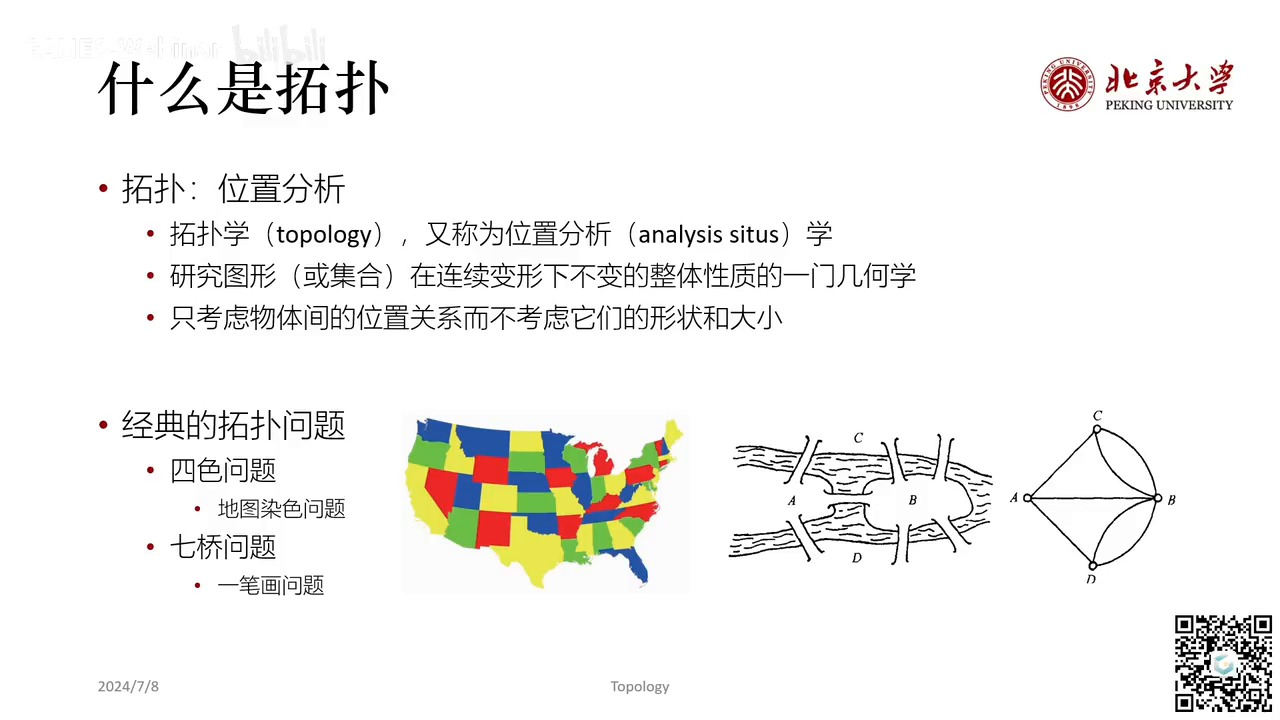
\includegraphics[width=0.92\textwidth]{figures/fig_02_what.jpg}
\caption{什么是拓扑：位置分析与两个经典问题\vtag}
\end{figure}
\srcnote{00:06:30--00:06:45}
\end{minipage}


拓扑学（topology）又称为位置分析（analysis situs）学。讲者解释，位置分析的意思是只关心图形的位置，与度量相关的内容，比如形状和大小，暂时不在考虑范围。最关键的是图形之间的相对位置关系，而这种位置关系可以包含图形的连续变形。拓扑研究图形（或集合）在连续变形下不变的整体性质，所以本质上拓扑也是几何学的一部分。

\subsection{四色问题}

最经典的拓扑问题相信大家一定接触过。四色问题又称为地图染色问题：给一张地图上的每个省份涂色，保证相邻的两个省份颜色一定不同，最少需要多少种颜色？这个问题已经被证明了是四种颜色。

\begin{knowledgebox}{四色定理的证明}
讲义作者补充：四色定理在 1976 年由 Appel 与 Haken 借助计算机穷举大量构形给出证明，是第一个主要依赖计算机完成的著名定理证明。它是一个“拓扑”问题，因为答案只取决于哪些区域相邻，而与区域的形状和大小无关。
\end{knowledgebox}

\subsection{七桥问题}

类似的还有七桥问题，也就是大家在小学奥数里见过的一笔画问题：给定一张图，能否一笔把它画出来，即图上的任何一条边都不会被重复经过两次。它最早来源于欧拉思考的问题：城市里有七座桥，能否不重复地正好用一条路线走遍这七座桥。

讲者说这个问题的解答也很简单，直接去看图上每个节点的度数就可以了：偶数度的节点不影响答案，奇数度的节点必须是两个或者零个，只有这种情况下才能一笔画完整个图形，或者说走过这七座桥。

\begin{knowledgebox}{一笔画的判定}
讲义作者补充：对一个连通图，设 $d(v)$ 为节点 $v$ 的度数。由于每条边贡献两个端点，
\begin{equation*}
\sum_vd(v)=2|E|,
\end{equation*}
所以奇数度节点的个数一定是偶数。一笔画存在当且仅当奇数度节点有零个（此时可以回到起点）或两个（此时必须从一个奇数度节点出发，到另一个结束）。哥尼斯堡七桥对应的图四个节点都是奇数度，所以无解。
\end{knowledgebox}

\section{同胚}

\noindent\begin{minipage}{\textwidth}
\begin{figure}[H]
\centering
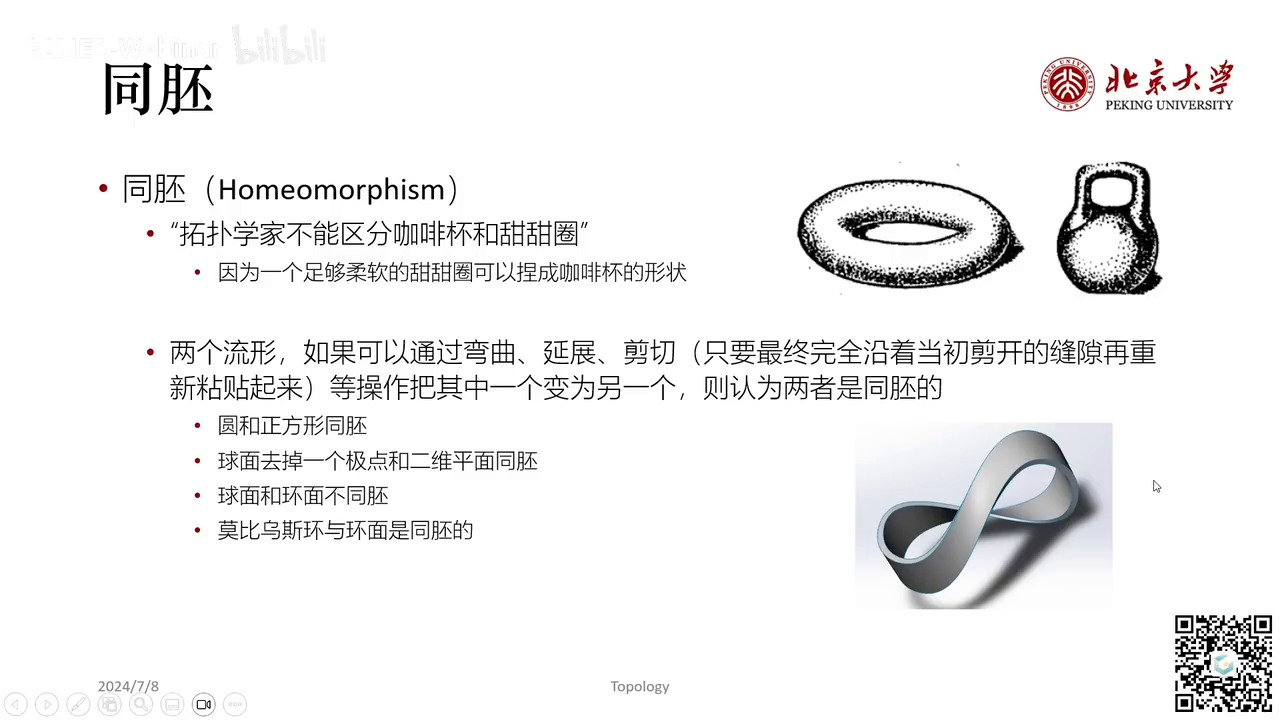
\includegraphics[width=0.92\textwidth]{figures/fig_03_homeo.jpg}
\caption{同胚：咖啡杯与甜甜圈，以及莫比乌斯环\vtag}
\end{figure}
\srcnote{00:10:15--00:10:30}
\end{minipage}


数学上有一个笑话：拓扑学家不能区分咖啡杯和甜甜圈。为什么呢？因为一个足够柔软的甜甜圈可以捏成咖啡杯的形状。讲者解释：课件右边的图虽然不是咖啡杯，但可以看成是把咖啡杯的把手朝上拎起来的样子。想象甜甜圈是橡皮泥做成的，你可以去捏橡皮泥的任何地方，把它捏成别的形状，但你不能把不相连的两处粘在一起，也不能在橡皮泥中间挖洞。

两个流形，如果可以通过弯曲、延展、剪切（只要最终完全沿着当初剪开的缝隙再重新粘贴起来）等操作把其中一个变为另一个，则认为两者是同胚的（homeomorphism）。

\begin{knowledgebox}{同胚的严格定义}
讲义作者补充：两个拓扑空间 $X,Y$ 同胚，是指存在一个双射 $\varphi:X\to Y$，它本身连续，并且逆映射也连续。“剪开后沿原缝隙粘回”之所以允许，是因为最终得到的映射在每个点附近仍然是连续的；而真正“粘上”或“挖洞”会改变哪些点彼此邻近，破坏了连续性。
\end{knowledgebox}

一些最简单的例子：
\begin{itemize}
\item 圆和正方形同胚：把正方形的四个角揉一揉，揉成圆形。
\item 球面去掉一个极点和二维平面同胚。讲者解释：球面可以用球坐标 $(\theta,\phi)$ 参数化，但极点处的参数是退化的；去掉一个极点后，可以想象从底下把球挖开，把它揉一揉、摊开成平面。
\item 球面和环面不同胚：环面就是甜甜圈的表面。
\item 课件上还说莫比乌斯环与环面同胚，见下面的提醒。
\end{itemize}

\begin{knowledgebox}{球面去掉一点同胚于平面}
讲义作者补充：一个具体的同胚是球极投影。把单位球放在平面上，从北极 $N$ 向球面上任意一点 $P\ne N$ 作射线，射线与平面的交点就是 $P$ 的像。对单位球 $x^2+y^2+z^2=1$，从北极 $(0,0,1)$ 投影到平面 $z=0$，公式为
\begin{equation*}
(x,y,z)\mapsto\left(\frac{x}{1-z},\ \frac{y}{1-z}\right),
\end{equation*}
它连续、可逆且逆映射连续。越接近北极的点被投到越远的地方，北极本身对应“无穷远点”。
\end{knowledgebox}

\begin{warningbox}{莫比乌斯环与环面并不同胚}
课件写道“莫比乌斯环与环面是同胚的”，讲者给出的理由是把圆环剪开、扭转 $180$ 度再接上。讲义作者提醒：这一步违反了同胚定义中“沿原缝隙重新粘回”的要求，扭转后再粘是不同的粘法。事实上二者不同胚：莫比乌斯环有边界，且不可定向；环面没有边界，并且可定向。讲者接着说的莫比乌斯环“无法区分内外”，恰恰是它与环面不同的拓扑性质。
\end{warningbox}

讲者介绍，莫比乌斯环是一种非常著名的拓扑结构，它有很重要的性质：无法区分内外，两个面是等同的，没有内和外的概念。沿着莫比乌斯环走一圈下来，可以正好走遍它上面的每一块地方。

\section{亏格}

\noindent\begin{minipage}{\textwidth}
\begin{figure}[H]
\centering
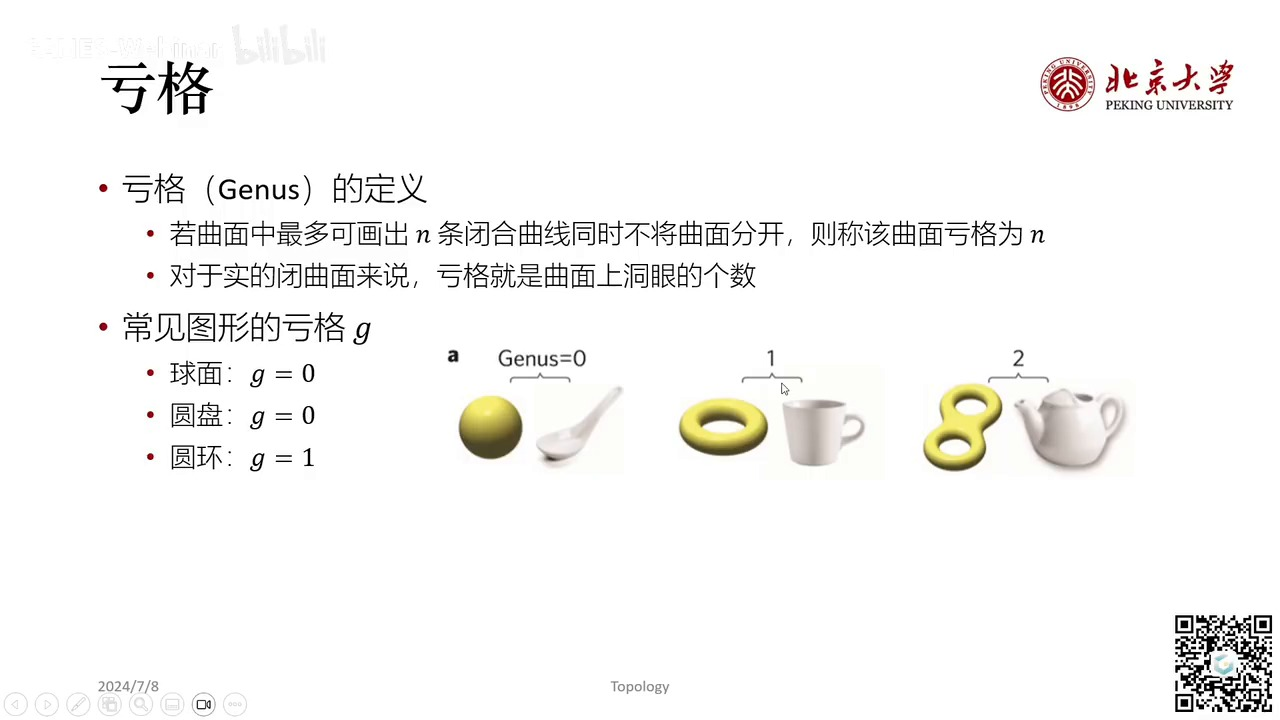
\includegraphics[width=0.92\textwidth]{figures/fig_04_genus.jpg}
\caption{亏格：曲面上“洞”的个数\vtag}
\end{figure}
\srcnote{00:11:30--00:11:45}
\end{minipage}


亏格（genus）的定义是：若曲面中最多可画出 $n$ 条闭合曲线同时不将曲面分开，则称该曲面亏格为 $n$。对于实的闭曲面来说，亏格就是曲面上洞眼的个数。

讲者举例：在平面上，随便画一条闭曲线一定会将平面分开，所以亏格是零。再看甜甜圈，在甜甜圈上画一条闭合曲线可以不将它分开，比如沿着甜甜圈的一圈剪开，剪完以后变成了圆柱形，还是连在一起的，所以甜甜圈的亏格是一。常见图形的亏格：球面上没有洞，$g=0$；圆盘也没有洞，$g=0$；课件上的“圆环”指环面，$g=1$；课件最右边有两个洞的曲面，$g=2$。

\begin{warningbox}{“圆环”在这里指环面}
课件上写“圆环：$g=1$”，讲者也说圆环和甜甜圈是同胚的。讲义作者提醒：这里的“圆环”应理解为环面，也就是甜甜圈的表面。如果“圆环”指的是平面上两个同心圆之间的环形区域，它与环面并不同胚，它的亏格是零，只是有两条边界。
\end{warningbox}

\section{闭曲面分类与三角剖分}

\subsection{闭曲面分类定理}

\noindent\begin{minipage}{\textwidth}
\begin{figure}[H]
\centering
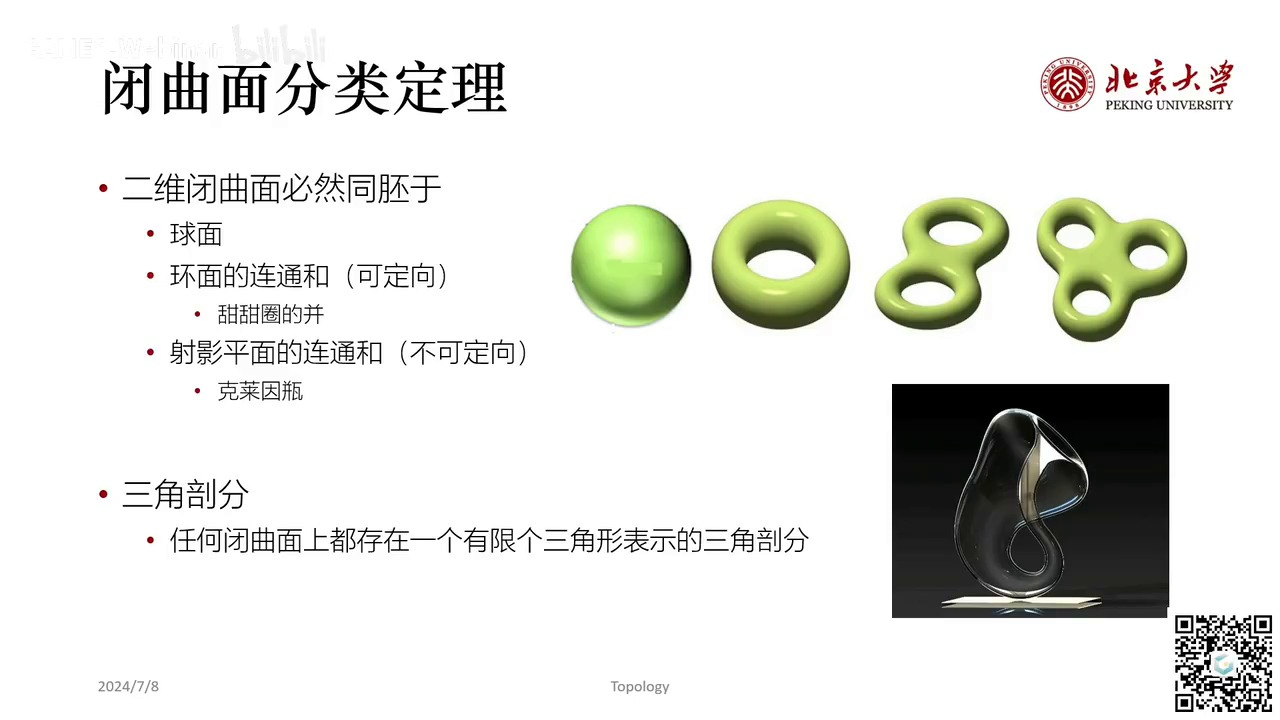
\includegraphics[width=0.92\textwidth]{figures/fig_05_classification.jpg}
\caption{闭曲面分类定理：球面、环面的连通和、射影平面的连通和\vtag}
\end{figure}
\srcnote{00:14:30--00:14:45}
\end{minipage}


基于亏格的定义，拓扑学上又形成了闭曲面分类定理。讲者说这是很神奇的性质：所有的二维闭曲面必然同胚于下面三类之一：
\begin{itemize}
\item 球面；
\item 环面的连通和（可定向），也就是若干个甜甜圈的并。连通和的意思是把它们并在一起，同时保证结果是连通的，比如课件上并在一起的两个和三个甜甜圈；
\item 射影平面的连通和（不可定向），例如克莱因瓶。
\end{itemize}

讲者解释不可定向曲面：甜甜圈有内外之分，而克莱因瓶没有内外之分。课件右下角的克莱因瓶看起来有一个开口，但从开口往里面倒水，会发现它只有一个面，内部的面和外部的面是连通在一起的。它不像平常的柱形水壶，你在里面转不会转到外面来。这种曲面一般比较少见，研究中一般考虑前两种，所以可以大致认为：你关心的二维闭曲面，要么是球面，要么是环面的连通和。

\begin{knowledgebox}{亏格和连通和}
讲义作者补充：$g$ 个环面的连通和就是亏格为 $g$ 的可定向闭曲面，记作 $\Sigma_g$；球面可以看成 $g=0$ 的情形。所以对可定向闭曲面而言，“同胚”这个看似复杂的问题被一个整数 $g$ 完全决定：两个可定向闭曲面同胚，当且仅当它们的亏格相同。
\end{knowledgebox}

\subsection{三角剖分}

闭曲面还有三角剖分的定理：任何闭曲面上都存在一个由有限个三角形表示的三角剖分。讲者说，在图形学里我们一般都把曲面变成三角网格，而三角网格就是对曲面的三角剖分。这个定理保证了用三角网格去分析的方法适用于任何闭曲面。大家平时用的时候可能没有想过为什么曲面天然就可以剖分成三角形，但从理论上说，这是有定理对应着的。

\section{欧拉示性数}

\subsection{定义}

\noindent\begin{minipage}{\textwidth}
\begin{figure}[H]
\centering
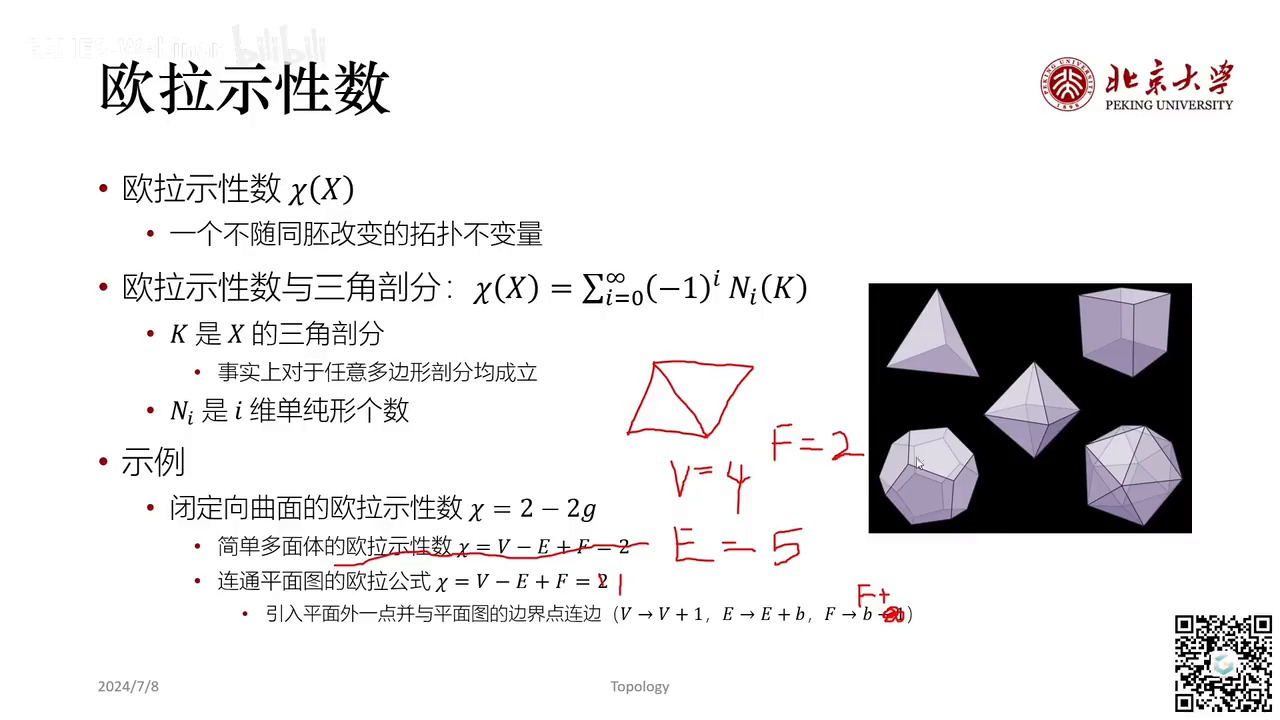
\includegraphics[width=0.92\textwidth]{figures/fig_06_euler.jpg}
\caption{欧拉示性数与三角剖分\vtag}
\end{figure}
\srcnote{00:21:00--00:21:15}
\end{minipage}


有了亏格和三角剖分的概念以后，再来看欧拉示性数。欧拉示性数 $\chi(X)$ 是一个不随同胚改变的拓扑不变量：不管是咖啡杯还是甜甜圈，同胚的两个东西欧拉示性数一定相同。它与三角剖分的关系是
\begin{equation}
\chi(X)=\sum_{i=0}^{\infty}(-1)^iN_i(K),
\end{equation}
其中 $K$ 是 $X$ 的三角剖分（事实上对于任意多边形剖分均成立），$N_i$ 是 $i$ 维单纯形的个数。

讲者解释：比如三维空间中有一个二维曲面，给它做三角剖分。剖分完以后，零阶单纯形是点，一阶单纯形是三角形的边，二阶单纯形是三角形本身。所以对二维曲面来说，欧拉示性数就等于三角剖分的点数减去边数加上面数：
\begin{equation}
\chi=|V|-|E|+|F| .
\end{equation}

\subsection{与亏格的关系}

对于任何闭定向曲面，欧拉示性数一定满足
\begin{equation}
\chi=2-2g,
\end{equation}
其中 $g$ 是亏格。比如球面的亏格是零，所以它的欧拉示性数是 $2-0=2$。

讲者说，由于任何简单多面体都同胚于球面，所以对任何简单多面体都有
\begin{equation}
|V|-|E|+|F|=2 ,
\end{equation}
这就是欧拉公式。大家可能会觉得 $V,E,F$ 怎么组合是要背的，但接触了欧拉示性数的概念之后，就不用背了。如果给定的是三维的图形，做四面体剖分，仍然是点数减边数加面数再减体数，结果还是 $1$（实心的球）。

\begin{warningbox}{实心体的欧拉示性数}
讲者口头上说对四面体剖分“还是等于二”。讲义作者按定义核对：对实心球的四面体剖分，$\chi=|V|-|E|+|F|-|T|$，其中 $|T|$ 是四面体个数，结果是 $1$ 而不是 $2$。例如单个四面体有 $4$ 个点、$6$ 条边、$4$ 个面、$1$ 个体，$4-6+4-1=1$。等于 $2$ 的是它的表面（球面），实心球与一个点同伦，欧拉示性数是 $1$。
\end{warningbox}

\subsection{例子：立方体与平面图}

\noindent\begin{minipage}{\textwidth}
\begin{figure}[H]
\centering
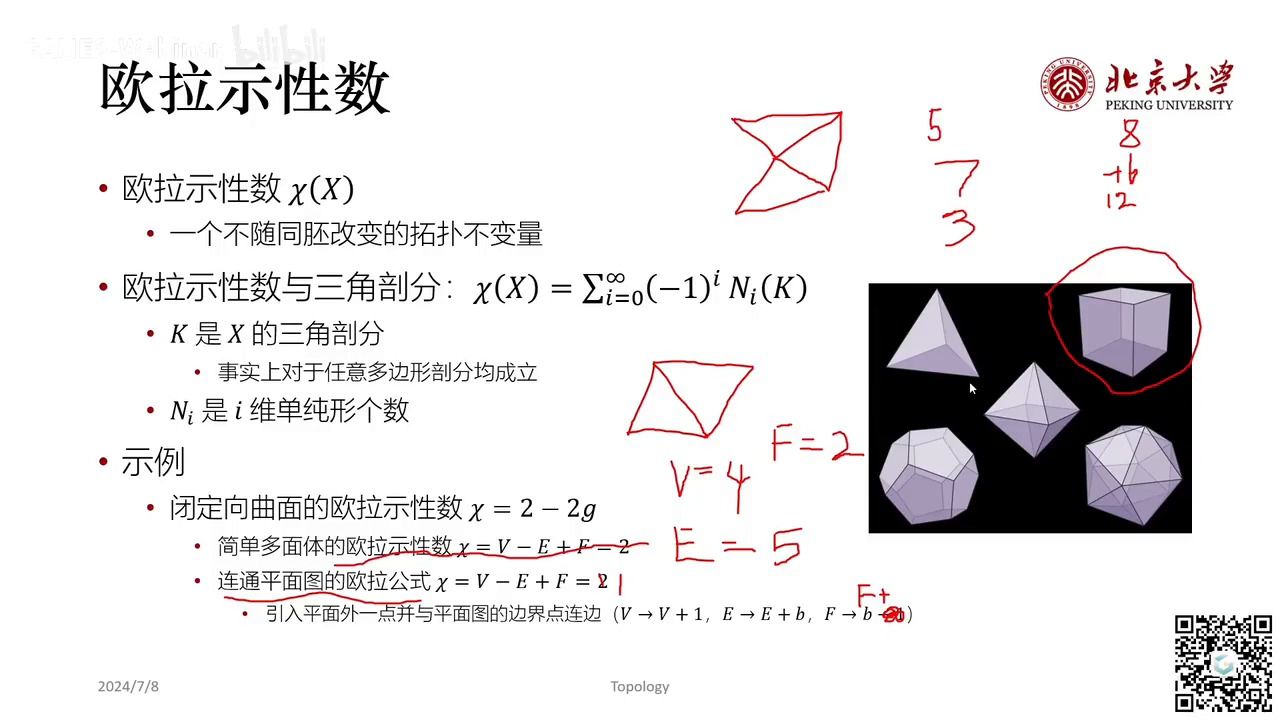
\includegraphics[width=0.92\textwidth]{figures/fig_07_euler2.jpg}
\caption{欧拉示性数的例子：立方体与连通平面图\vtag}
\end{figure}
\srcnote{00:22:45--00:23:00}
\end{minipage}


讲者用立方体验证：它有 $8$ 个顶点、$6$ 个面、$12$ 条边，$8+6-12=2$，满足简单多面体的欧拉公式。

从简单多面体的欧拉公式还可以推导出连通平面图的欧拉公式。课件上的做法是：在平面外引入一点，并将它与平面图边界上的点连边。设边界上有 $b$ 个点，那么
\begin{equation}
|V|\to|V|+1,\qquad |E|\to|E|+b,\qquad |F|\to|F|-1+b .
\end{equation}
讲者说这样就变成了简单多面体，而点数加一、面数加 $b-1$、边数加 $b$，所以 $|V|-|E|+|F|$ 没有变。于是对连通平面图也有 $|V|-|E|+|F|=2$，前提是把平面图边界外的区域也算作一个面。

讲者在白板上举了两个例子：一个四边形中间加一条对角线，有 $4$ 个顶点、$5$ 条边，内部有 $2$ 个面；再加一个点，有 $5$ 个顶点、$7$ 条边，内部有 $3$ 个面。只数内部的面时，$4-5+2=1$，$5-7+3=1$；把外部区域也算作一个面，就都等于 $2$。

\begin{practicebox}{用欧拉公式检查三角网格}
讲义作者补充：对闭合的三角网格，每个三角形有三条边，每条边被两个三角形共享，所以 $3|F|=2|E|$。代入 $|V|-|E|+|F|=2-2g$ 得到
\begin{equation*}
|E|=3|V|-6+6g,\qquad |F|=2|V|-4+4g .
\end{equation*}
因此大网格中面数约为点数的 $2$ 倍，边数约为点数的 $3$ 倍，每个顶点平均连接约 $6$ 条边。读者可以用这个关系检查一个网格是否闭合，或者由点、边、面的个数算出网格的亏格。
\end{practicebox}

\section{卷绕数与回转数}

\noindent\begin{minipage}{\textwidth}
\begin{figure}[H]
\centering
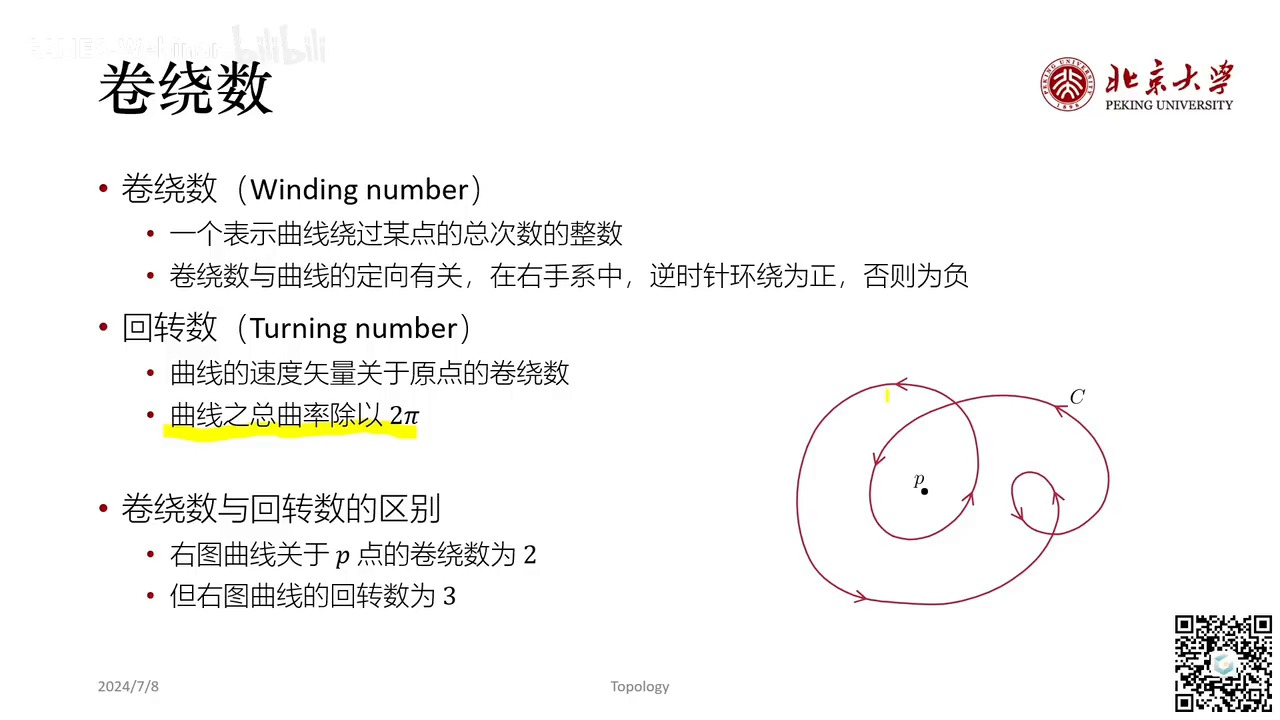
\includegraphics[width=0.92\textwidth]{figures/fig_08_winding.jpg}
\caption{卷绕数与回转数的区别\vtag}
\end{figure}
\srcnote{00:24:15--00:24:30}
\end{minipage}


卷绕数（winding number）是表示曲线绕过某点的总次数的整数。它与曲线的定向有关：在右手系中，逆时针环绕为正，顺时针环绕为负。讲者解释：逆时针绕一圈，卷绕数加一；顺时针绕一圈，卷绕数减一。

回转数（turning number）则是曲线的速度矢量，也就是切线方向关于原点的卷绕数，也可以把它看成曲线的总曲率除以 $2\pi$：
\begin{equation}
\text{回转数}=\frac{1}{2\pi}\oint_C\kappa\,\mathrm{d}s .
\end{equation}

\begin{knowledgebox}{卷绕数的积分公式}
讲义作者补充：对不经过点 $p$ 的闭曲线 $C$，卷绕数可以写成曲线上的点相对 $p$ 转过的总角度除以 $2\pi$，即
\begin{equation*}
w(C,p)=\frac{1}{2\pi}\oint_C\mathrm{d}\theta=\frac{1}{2\pi i}\oint_C\frac{\mathrm{d}z}{z-p},
\end{equation*}
后一种是复分析中的写法。回转数则把被积的角度换成切线方向的角度。
\end{knowledgebox}

两者的区别：课件右图中，曲线关于 $p$ 点的卷绕数是 $2$，因为曲线绕 $p$ 转了一圈又转了一圈；但曲线的回转数是 $3$。讲者解释，回转数是把曲线上每点的曲率全部算出来积分再除以 $2\pi$，与 $p$ 点无关；而卷绕数必须取一个参考点，所以两者一般不相等。

\begin{importantbox}{卷绕数在图形学中的用途}
讲义作者补充：卷绕数是判断“点在形状内部还是外部”的稳健工具。对封闭曲线，内部点的卷绕数非零，外部点为零。对三维的三角网格也可以定义广义卷绕数，把每个三角形对查询点张成的立体角加起来除以 $4\pi$；即使网格有破洞或自交，它也能给出接近 $0$ 或 $1$ 的平滑结果，常用于网格内外判定和布尔运算。
\end{importantbox}

\section{若尔当曲线定理}

\noindent\begin{minipage}{\textwidth}
\begin{figure}[H]
\centering
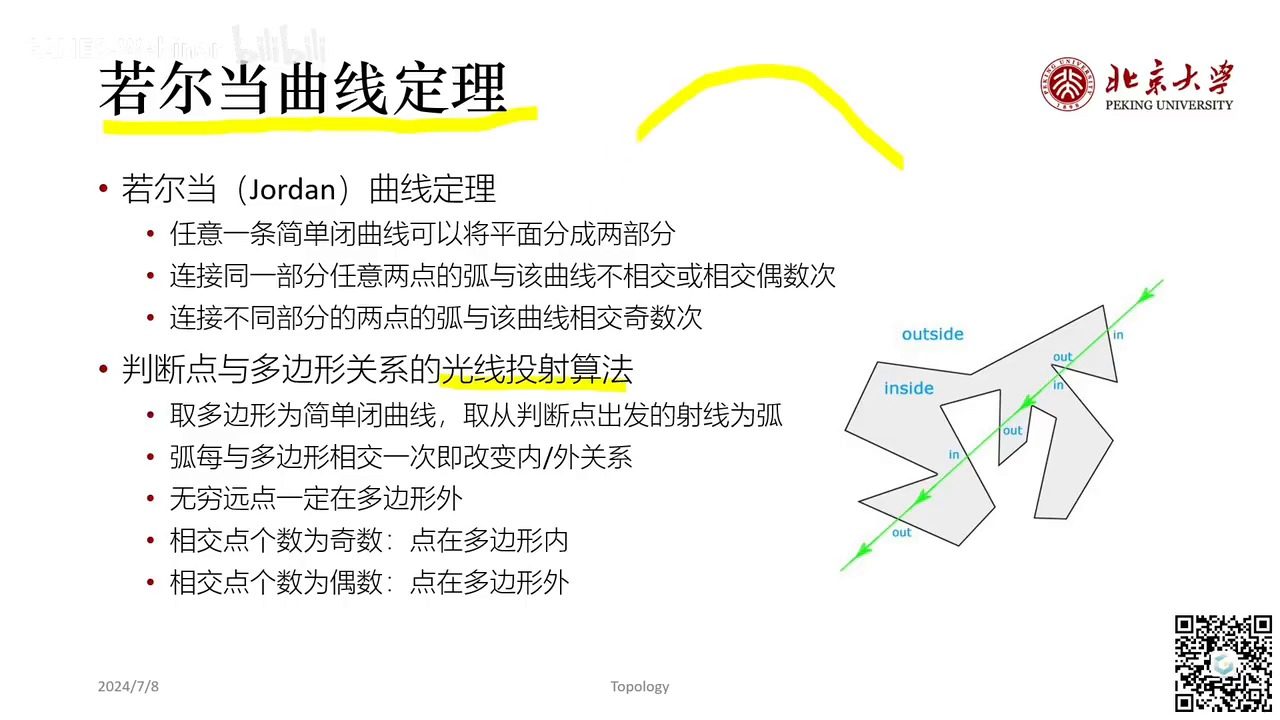
\includegraphics[width=0.92\textwidth]{figures/fig_09_jordan.jpg}
\caption{若尔当曲线定理与光线投射算法\vtag}
\end{figure}
\srcnote{00:25:00--00:25:15}
\end{minipage}


平面中的曲线还满足若尔当（Jordan）曲线定理，讲者说之前在计算几何那一讲已经讲过了，它是用光线投射判断点与多边形关系的理论基础。定理说：
\begin{itemize}
\item 任意一条简单闭曲线可以将平面分成两部分，也就是曲线内和曲线外；
\item 连接同一部分任意两点的弧与该曲线不相交或相交偶数次；
\item 连接不同部分的两点的弧与该曲线相交奇数次。
\end{itemize}

\noindent\begin{minipage}{\textwidth}
\begin{figure}[H]
\centering
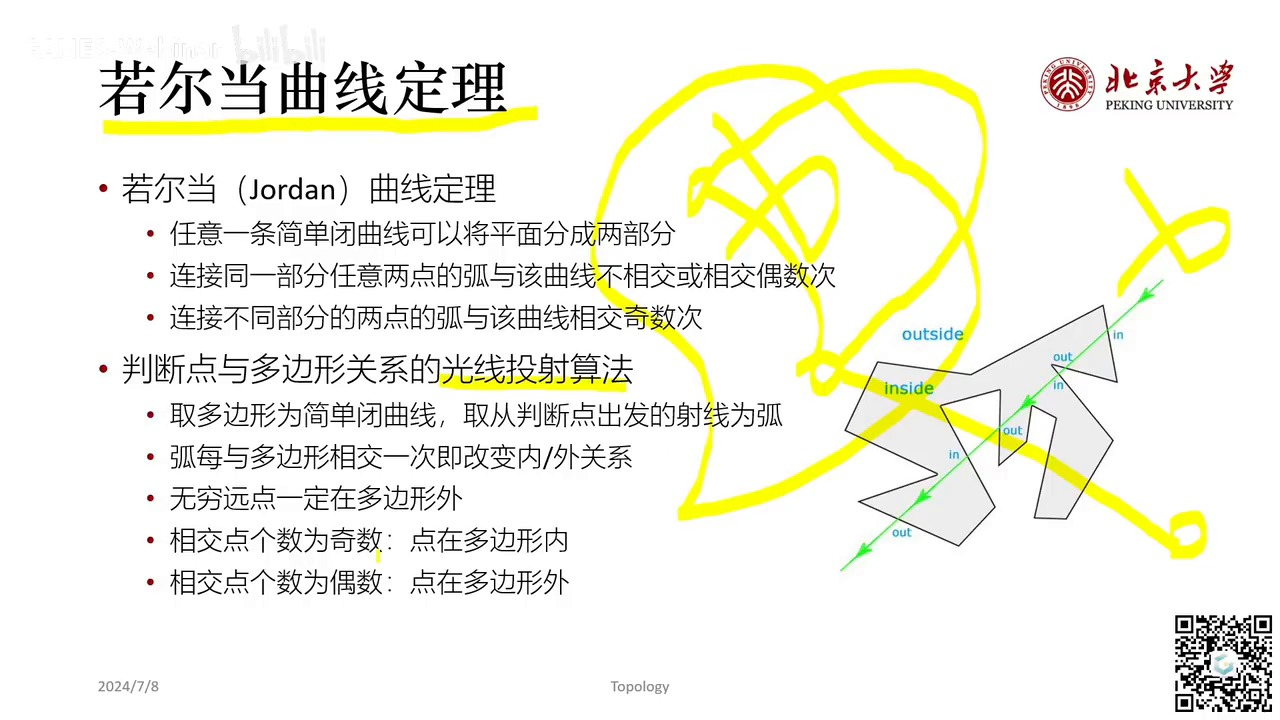
\includegraphics[width=0.92\textwidth]{figures/fig_10_jordan2.jpg}
\caption{讲者在课件上画出与曲线相交偶数次和奇数次的弧\vtag}
\end{figure}
\srcnote{00:26:00--00:26:15}
\end{minipage}


讲者在课件上随便画了一条曲线，它把屏幕分成两部分。连接同一部分的两点，可以画一条与曲线不相交的弧，也可以画一条相交两次的弧；而连接内部一点和外部一点的弧，一定与这条简单闭曲线相交奇数次。

因此有判断点与多边形关系的光线投射算法：
\begin{itemize}
\item 取多边形为简单闭曲线，取从判断点出发的射线为弧；
\item 弧每与多边形相交一次即改变内外关系；
\item 无穷远点一定在多边形外；
\item 相交点个数为奇数：点在多边形内；相交点个数为偶数：点在多边形外。
\end{itemize}

\begin{warningbox}{光线投射的退化情形}
讲义作者提醒：实现时射线可能恰好经过多边形的顶点或与某条边重合，此时简单地数交点会出错。常见的处理是对每条边采用“半开区间”规则，例如只在边的一个端点严格位于射线上方、另一个端点不在上方时才计数。对于自交的多边形，奇偶规则与非零卷绕数规则给出的“内部”也可能不同。
\end{warningbox}

\section{布劳威尔不动点定理}

\noindent\begin{minipage}{\textwidth}
\begin{figure}[H]
\centering
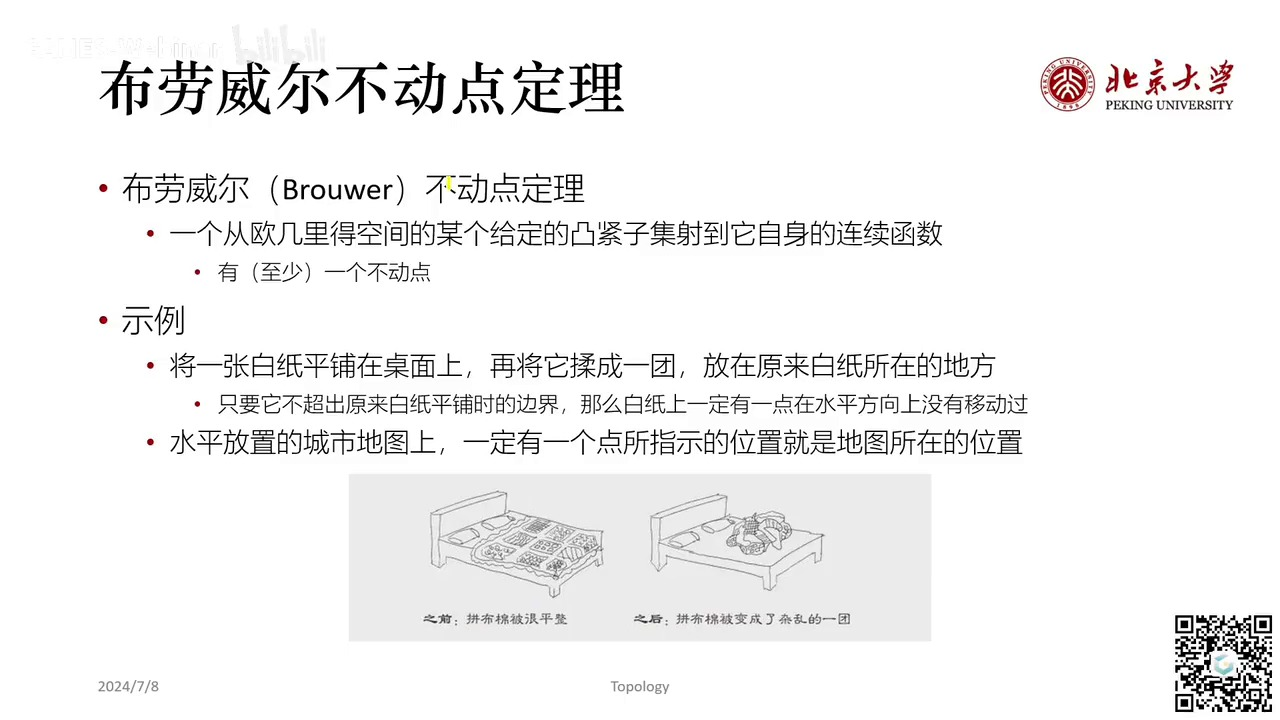
\includegraphics[width=0.92\textwidth]{figures/fig_11_brouwer.jpg}
\caption{布劳威尔不动点定理\vtag}
\end{figure}
\srcnote{00:26:15--00:26:30}
\end{minipage}


布劳威尔（Brouwer）不动点定理说：一个从欧几里得空间的某个给定的凸紧子集射到它自身的连续函数，有（至少）一个不动点。用公式写，若 $D\subset\mathbb R^n$ 是凸紧集，$f:D\to D$ 连续，则
\begin{equation}
\exists\,x^*\in D,\qquad f(x^*)=x^* .
\end{equation}

讲者用一些直观的例子理解。将一张白纸平铺在桌面上，再将它揉成一团，放在原来白纸所在的地方：只要它不超出原来白纸平铺时的边界，那么白纸上一定有一点在水平方向上没有移动过。

\noindent\begin{minipage}{\textwidth}
\begin{figure}[H]
\centering
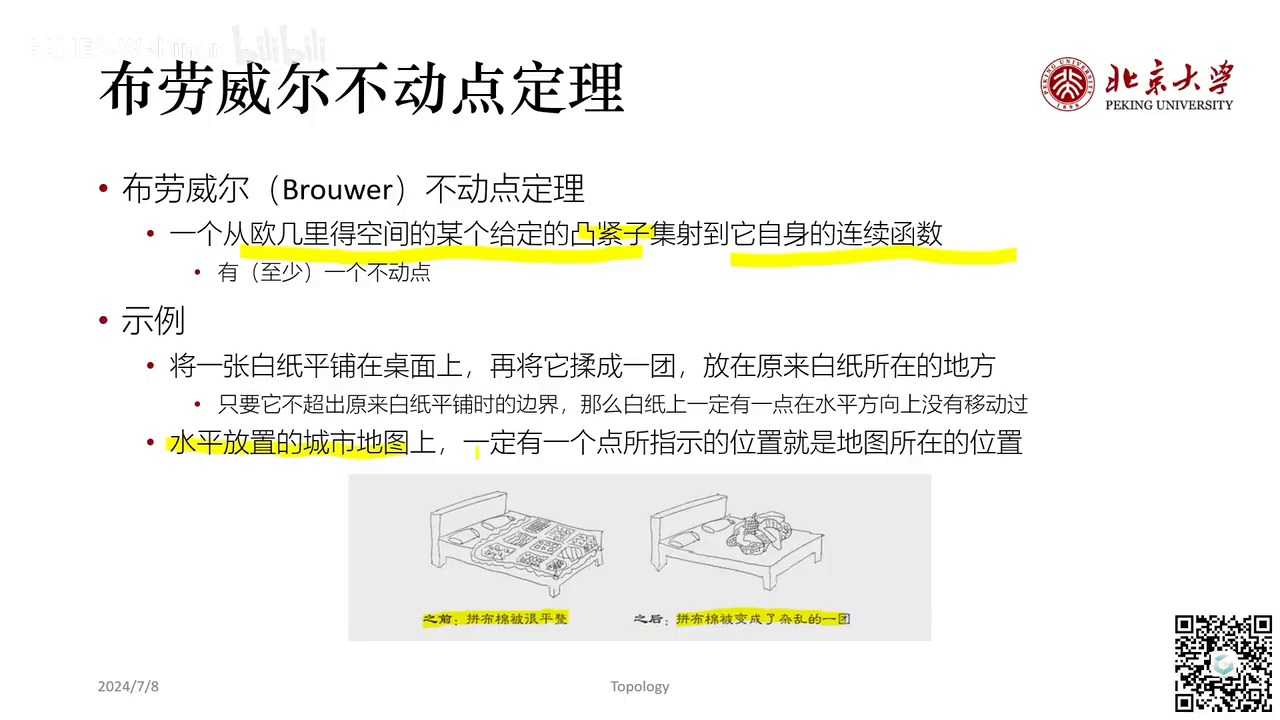
\includegraphics[width=0.92\textwidth]{figures/fig_12_brouwer2.jpg}
\caption{示例：铺平的床单与揉成一团的床单\vtag}
\end{figure}
\srcnote{00:27:30--00:27:45}
\end{minipage}


课件下面的图也是一样：一开始床上的被子是平整的，把被子变成杂乱的一团丢在床上，被子上必然有一个点，它相对于床的水平位置没有发生改变。

\noindent\begin{minipage}{\textwidth}
\begin{figure}[H]
\centering
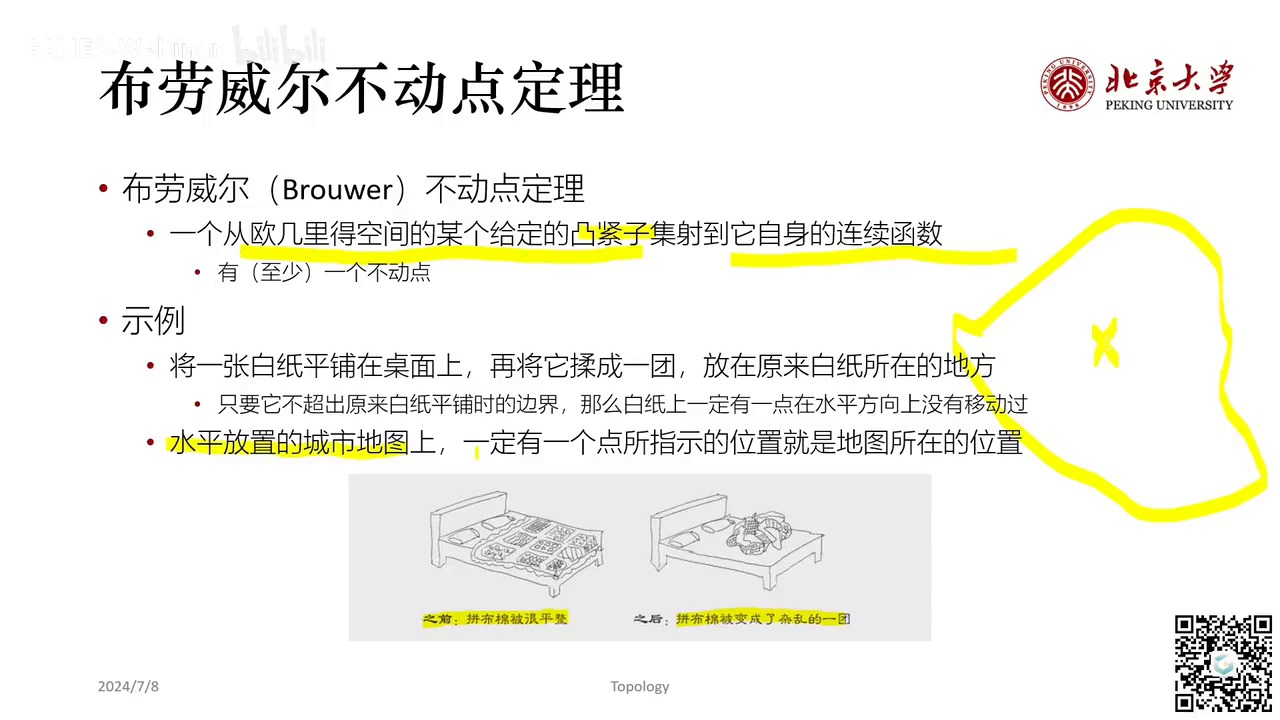
\includegraphics[width=0.92\textwidth]{figures/fig_13_brouwer3.jpg}
\caption{示例：水平放置的城市地图上一定有一个点指示的就是它自己所在的位置\vtag}
\end{figure}
\srcnote{00:28:15--00:28:30}
\end{minipage}


讲者说另一个例子说神奇也不神奇：在一张水平放置的城市地图上，一定有一个点所指示的位置就是地图所在的位置。首先找到你所在的位置大体落在地图上什么地方，地图上的点和它指示的点在精度要求的范围内就重合了；要更精细，就把那一块放大再找你在哪，你总是能找到。这样取极限之后，一定能找到指示的位置就是地图所在位置的那个点。

\begin{knowledgebox}{一维情形的证明}
讲义作者补充：在区间 $[a,b]$ 上，设 $f:[a,b]\to[a,b]$ 连续，令 $h(x)=f(x)-x$，则 $h(a)\ge 0$，$h(b)\le 0$，由介值定理存在 $x^*$ 使 $h(x^*)=0$。高维的证明需要用到拓扑工具，但思想相同：连续性加上“映回自身”就迫使某个点不动。这个定理在第十四讲提到的不动点迭代和博弈均衡的存在性中都有影子。
\end{knowledgebox}

\section{毛球定理}

\subsection{庞加莱--霍普夫定理}

\noindent\begin{minipage}{\textwidth}
\begin{figure}[H]
\centering
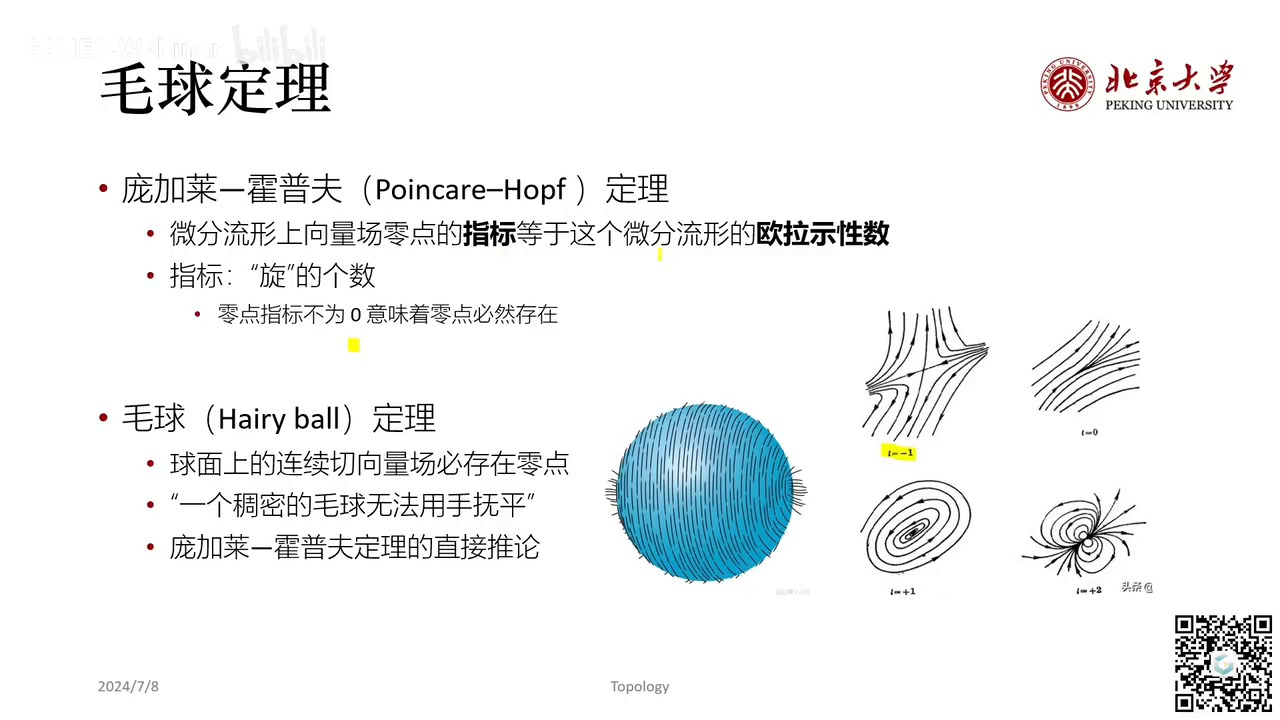
\includegraphics[width=0.92\textwidth]{figures/fig_14_hairy.jpg}
\caption{庞加莱--霍普夫定理与零点的指标\vtag}
\end{figure}
\srcnote{00:29:45--00:30:00}
\end{minipage}


毛球定理是庞加莱--霍普夫（Poincar\'e--Hopf）定理的推论，讲者说这个名字感觉怪可爱的。庞加莱--霍普夫定理说：微分流形上向量场零点的指标之和等于这个微分流形的欧拉示性数，
\begin{equation}
\sum_i\operatorname{ind}_{x_i}(v)=\chi(M).
\end{equation}

指标是什么意思？课件说是“旋”的个数。讲者看右下角的图：点附近有进有出、形成鞍形的，指标记作 $-1$；附近没有旋的点，指标是 $0$；点附近有一个旋，指标是 $+1$；附近有两个旋，指标是 $+2$。只要零点的指标不为零，就意味着零点必然存在。

\begin{warningbox}{是指标之和}
课件写的是“向量场零点的指标等于这个微分流形的欧拉示性数”。讲义作者提醒：严格的说法是所有零点（假设是孤立的）的指标之和等于欧拉示性数，单个零点的指标可以是 $-1$、$+2$ 等不同的值，只有加起来才等于 $\chi$。例如球面上可以有两个指标为 $+1$ 的零点（南北极），加起来是 $2$。
\end{warningbox}

\subsection{毛球定理}

\noindent\begin{minipage}{\textwidth}
\begin{figure}[H]
\centering
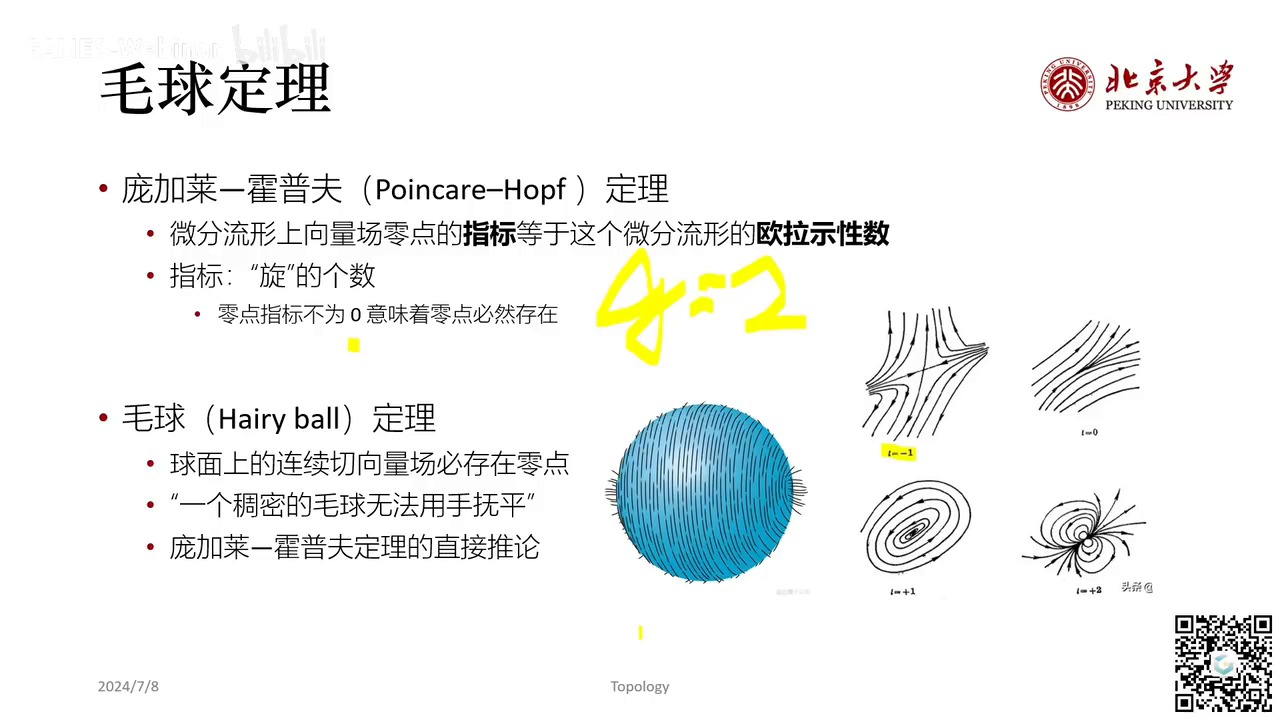
\includegraphics[width=0.92\textwidth]{figures/fig_15_hairy2.jpg}
\caption{毛球定理：一个稠密的毛球无法用手抚平\vtag}
\end{figure}
\srcnote{00:30:30--00:30:45}
\end{minipage}


毛球（hairy ball）定理说：球面上的连续切向量场必存在零点。它是上面定理的直接推论：球面的欧拉示性数 $\chi=2\ne 0$，所以指标之和不为零，零点必然存在。用直观的概念理解：毛球是长满毛的球，没有办法用手把它抚平，一定会有地方抚不平，毛还是戳出来的。讲者说现实生活中不存在处处都有毛并且能完全抚平的毛球。

\begin{importantbox}{毛球定理在图形学中的影响}
讲义作者补充：在曲面上设计方向场、十字场来引导四边形重网格化或纹理合成时，若曲面的 $\chi\ne 0$（比如任何亏格为零的闭曲面），场中就必然存在奇异点，它们的指标之和由 $\chi$ 决定。只有环面（$\chi=0$）上才可能有处处非零的光滑切向量场。所以奇异点不是算法的缺陷，而是拓扑的要求，算法能做的只是决定把它们放在哪里。
\end{importantbox}

\section{庞加莱猜想}

\noindent\begin{minipage}{\textwidth}
\begin{figure}[H]
\centering
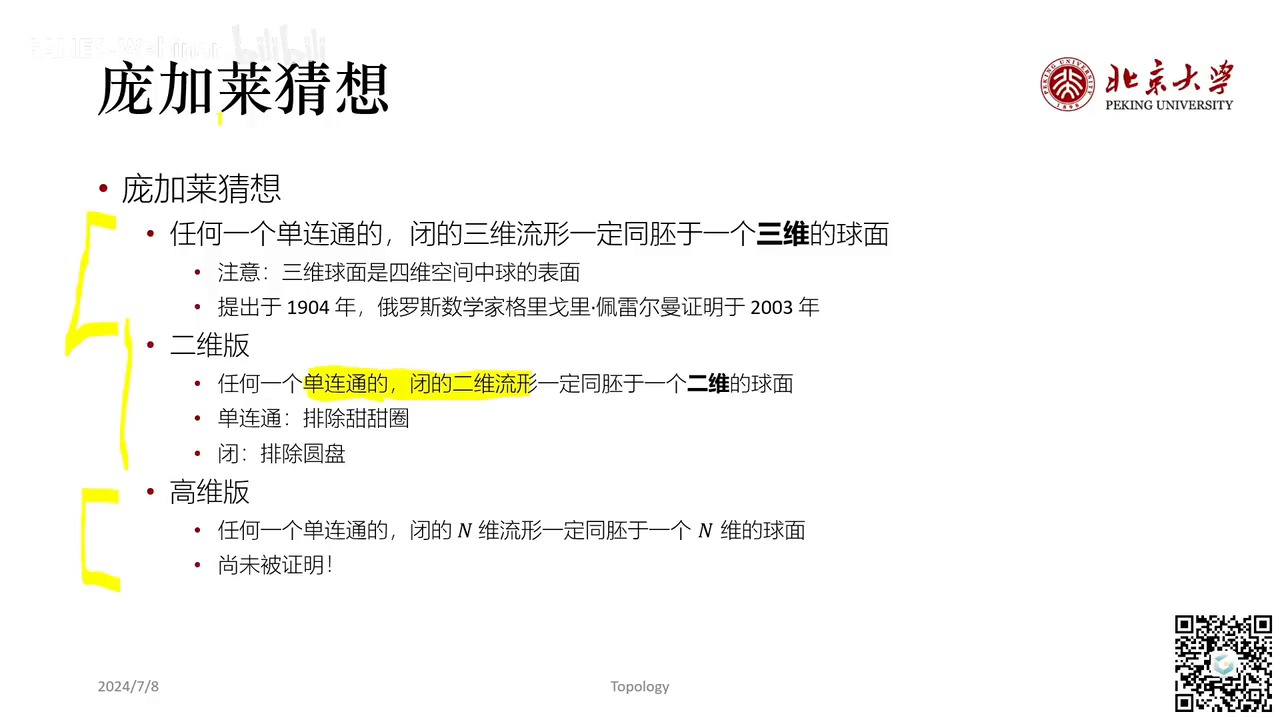
\includegraphics[width=0.92\textwidth]{figures/fig_16_poincare.jpg}
\caption{庞加莱猜想及其二维和高维版本\vtag}
\end{figure}
\srcnote{00:33:15--00:33:30}
\end{minipage}


最后是庞加莱猜想：任何一个单连通的、闭的三维流形一定同胚于一个三维的球面。讲者提醒，三维球面是四维空间中球的表面。这个猜想于 1904 年由庞加莱提出，2003 年由俄罗斯数学家格里戈里·佩雷尔曼证明，时隔大约一百年。

这个定理的低维版本可能更容易理解。二维版：任何一个单连通的、闭的二维流形一定同胚于一个二维的球面。讲者解释：既然要求单连通，就不能是甜甜圈，因为单连通不允许中间有洞；要求闭，就排除了圆盘。剩下的只有球面。

\begin{knowledgebox}{单连通}
讲义作者补充：一个空间是单连通的，是指它连通，并且其中任何一条闭曲线都可以在空间内连续地收缩成一个点。在球面上任何橡皮筋都能滑下来缩成一点；而在环面上，绕着洞的那条橡皮筋怎样都缩不成一点，所以环面不是单连通的。
\end{knowledgebox}

课件还给出了高维版本：任何一个单连通的、闭的 $N$ 维流形一定同胚于一个 $N$ 维的球面，并写着“尚未被证明”。

\begin{warningbox}{高维庞加莱猜想已被证明}
讲义作者提醒：课件的高维版本表述过于简化，结论也需要更正。高维情形的正确表述需要比“单连通”更强的条件（与球面同伦等价）；在这个表述下，$N\ge 5$ 的情形由 Smale 在 1961 年证明，$N=4$ 的情形由 Freedman 在 1982 年证明，再加上 2003 年完成的三维情形，拓扑意义下的广义庞加莱猜想在所有维数都已成立。仅要求单连通是不够的，例如两个二维球面的乘积是单连通的闭四维流形，但它不同胚于四维球面。
\end{warningbox}

\section{结语}

讲者说，以上就是今天关于拓扑的简要介绍。这节课讲完以后，整个 GAMES001 系列也就到此为止了。本次课程因为只是普及性的课程，所以没有作业；之前布置了作业的课程，助教团队也已经在批改，批改结果会通过公众号和 QQ 群通知，并按照课程开始前的安排，给作业完成得比较好的同学一些小礼品。欢迎大家在 QQ 群里继续交流图形学和数学相关的知识。

回顾整个系列，从线性代数、概率论、优化一直讲到拓扑，这些数学工具在图形学中反复出现。拓扑这一讲提供的是一种整体的视角：亏格和欧拉示性数告诉我们网格的连接方式有怎样的约束，卷绕数和若尔当曲线定理支撑着内外判定，不动点定理和毛球定理则告诉我们某些东西必然存在，设计算法时不必徒劳地去消除它们。

\begin{practicebox}{自测}
\begin{enumerate}
\item 说明为什么哥尼斯堡七桥问题无解，并写出一笔画存在的条件。
\item 一个亏格为 $2$ 的闭三角网格有 $1000$ 个顶点，它有多少条边和多少个三角形？
\item 举出课件中曲线的卷绕数与回转数不同的原因。
\item 用光线投射法判断点在多边形内外时，射线恰好经过顶点该怎样处理？
\item 用毛球定理解释为什么地球表面上任意时刻一定存在某个风速为零的地方。
\end{enumerate}
\end{practicebox}

\end{document}
